\documentclass[11pt]{article}
\usepackage{fancyhdr}
\usepackage{graphicx}
\usepackage{amssymb,amsmath}
\usepackage{psfrag}
\usepackage{color}
\usepackage[colorlinks]{hyperref}
\usepackage[footnotesize,hang,bf]{caption}
\usepackage{subeqnarray}
% \usepackage{amsthm}
 \usepackage{enumitem}
 \graphicspath{{Figures/}}
 \usepackage{multicol}
 \usepackage{ marvosym }
 \usepackage{wasysym}
 \usepackage{tikz}
 \usetikzlibrary{patterns}

 \newcommand{\ds}{\displaystyle}
 \DeclareMathOperator{\sech}{sech}

%%%%%%%%%%%%%%%%%%%%%%%%%%%%%%%%%%%%%%%%%%%%%%%%%%%%%%%%%%%%%%%%%%%%%%%%%%%%%%%%%%

\def\hwnum{4}
\def\term{Spring 2018}

\setlength{\oddsidemargin}{0 in}
\setlength{\evensidemargin}{0 in}
\setlength{\topmargin}{0.0 in}
\setlength{\textwidth}{6.45 in}
\setlength{\textheight}{8.5 in}
%\setlength{\headheight}{1 in}
\renewcommand{\baselinestretch}{0.95}

\pagestyle{fancy}
\rhead{ME 257/357\\ \term \\Problem Set \#\hwnum }
\lhead{}
\renewcommand{\headrulewidth}{0pt}

\begin{document}

\begin{center}
{\Large\bf ME 257/357 Gas Turbine Design: Problem Set \#\hwnum\\
       Due: Thursday, 5/31/2018 (before lecture)}
\end{center}

%=======================================================================================================
Before solving this problem set, outline the approach you want to follow. Provide all solution steps, and clearly mark your solution. Start with the general formulation, and simplify all expressions as much as possible. Plug in all numbers only at the end. Make and state necessary assumptions that you
think are required for solving the problem. You are encouraged to discuss the approach you want to follow on a conceptual level in groups; however, you have to submit your own write-up, plots, and non-trivial source code.
\\
\hrule
%=======================================================================================================
\vspace{2mm}
\noindent

\section*{Problem Formulation}

  In this assignment, we will analyze a compressor that is representative of the compressor stages found in the GE Honda HF-120 engine (shown in Fig.~\ref{FIG_CUTAWAY} below). Note that the compressor of the HF-120 consists of two low-pressure axial stages and one high-pressure centrifugal stage. However, we will consider only axial compressor stages and perform the analysis focusing on values of overall pressure ratio and thrust.

  \begin{figure}[!ht!]
      \begin{center}
          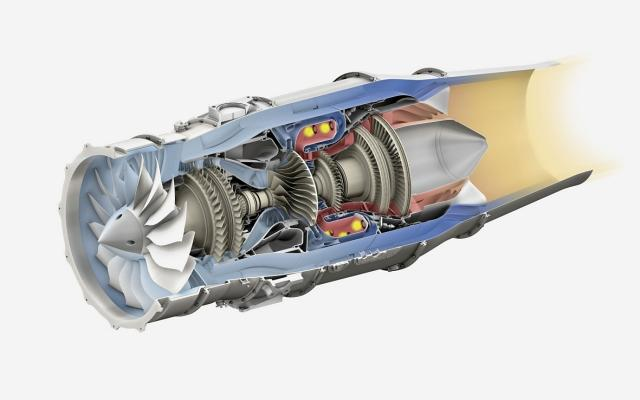
\includegraphics[width=0.9\textwidth]{GE_Honda_HF-120_Cutaway.jpg}
          \caption{\label{FIG_CUTAWAY} GE Honda HF-120 Engine Cutaway Drawing (from janes.ihs.com)}
      \end{center}
  \end{figure}

%%%%%%%%%%%%%%%%%%%%%%%%%%%%%%%%%%%%%%%%%%%%%%%%%%%%%%%%%%%%%%%%%%%%%%%%%%%%%%%%  
\section{Velocity Triangle}
  Consider a single compressor stage shown schematically in Fig.~\ref{FIG_SCHEMATIC}. At the mean radius (labeled in part a of the figure, $r_m$ = 30 cm), a cross-sectional cut (part b) shows the blade configuration. Assume that air angles and blade angles are the same.

  Use a value of 0.9 for the stage adiabatic efficiency. The axial velocity component at the design flow rate is 125 m/s, and the inlet air is at 1 atm and 20$^\circ$C.
  
  \begin{enumerate}[label=(\alph*)]
  	\item
    	If the hub-tip radius ratio is 0.8, would you expect the approximation of using mean radius to be very accurate?  Explain your reasoning.
    \item
    	Sketch velocity triangles (or, absolute and relative velocities) at the four locations between compressor elements: upstream of the IGV, between IGV and rotor, between rotor and stator, and downstream of the stator.
    \item
    	What is the power required to drive this single stage?  What should the shaft rotational speed be at these conditions?
  \end{enumerate}

  \begin{figure}[!ht!]
      \begin{center}
          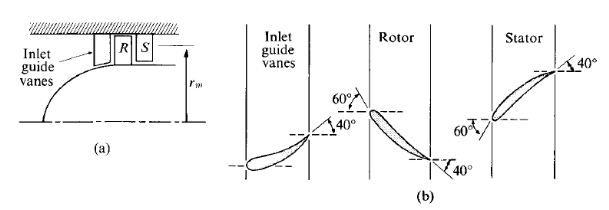
\includegraphics[width=0.9\textwidth]{schematic.png}
          \caption{\label{FIG_SCHEMATIC} Single-stage compressor with inlet guide vanes}
      \end{center}
  \end{figure}
%%%%%%%%%%%%%%%%%%%%%%%%%%%%%%%%%%%%%%%%%%%%%%%%%%%%%%%%%%%%%%%%%%%%%%%%%%%%%%%%  
\section{Compressor Map}
	In this problem we will construct a compressor map containing contour lines of constant $T_{04}/T_{02.5}$, $N/\sqrt{T_{02.5}}$, and overall compressor adiabatic efficiency $\eta_c$. Also, label the surge line and omit the curves above/left of the surge line. Note that we are using station 2.5 as a reference since this analysis is for the HPC section between stations 2.5 and 3.
    
    To simplify our analysis, we will represent the HF-120 compressor (two axial stages and one centrifugal stage) as \textbf{four axial stages}. Use the angles $\alpha_1$ = 30$^\circ$, $\alpha_2=60^\circ$ , $\beta_1=60^\circ$, $\beta_2 =30^\circ$, and the blade hub-to-tip-radius ratio is $r_\mathrm{hub}/r_\mathrm{tip}=0.6$.
    
	Consider the design condition at cruise altitude and speed (i.e., an altitude of 30,000 feet and at Mach 0.7). Let the reference axial velocity through compressor be $u_{x,\mathrm{ref}}=75$ m/s , and $U_\mathrm{ref}=307$ m/s. The stage adiabatic efficiency can be represented by the parabolic curve fit, 
    \begin{equation}
    	\eta_\mathrm{st}\left(\frac{u_x}{U}\right)=0.87-16\left(
        \frac{u_x}{U}-\frac{u_{x,\mathrm{ref}}}{U_\mathrm{ref}}\right)^2\ .
    \end{equation}
    The desired amount of maximum thrust at this operating condition is 3400 N, corresponding to $T_{04}=1600$ K.
    
    \textbf{Other engine specifications}: The fan pressure ratio is 2.0 and bypass ratio is 2.9. For an overall pressure ratio of 24, the design compressor pressure ratio is 12. Adiabatic efficiencies for the diffuser, fan, turbine, and nozzle are $\eta_d = 0.97 ,\ \eta_f = 0.92 ,\ \eta_t = 0.91 ,\ \eta_n = 0.98$, respectively.
Proceed as follows:
	\begin{enumerate}[label=(\alph*)]
    	\item
        	Determine the quantities $p_{03},\ \eta_\mathrm{st},\ T_{04},\ \dot{m}_a$, and $\bar{r}$ (the mean radius) at the design cruise operating condition described above. This will be ``Point A'' on the compressor map, and it will also give you an idea of what range of $u_x,\ T_{04}/ T_{02.5}$, and $N$ (shaft RPM) to consider for the map.
        \item
        	Do the values you found for size, $\bar{r}$ or $r_\mathrm{tip}$, and mass flow, $\dot{m}_a$, agree reasonably well with the HF-120 and quantities we have previously used?
         \item
         	Working symbolically, what is the relationship between $\eta_c$ and $\eta_\mathrm{st}$ ? Assume you would know operating conditions ($U$, $u_x$) blade angles ($\alpha_1,\ \beta_2$), stage efficiency $\eta_\mathrm{st}$, and the
number of stages $n$.
		\item
        	Calculate and plot the compressor map by completing the Matlab code in \emph{problemSet4Driver.m}, varying RPM from 15,000 to 30,000 and $u_x$ from 20 to 130. Also, show lines of constant $T_{04}/T_{02.5}$ and contours of $\eta_c$.
    \end{enumerate}
%%%%%%%%%%%%%%%%%%%%%%%%%%%%%%%%%%%%%%%%%%%%%%%%%%%%%%%%%%%%%%%%%%%%%%%%%%%%%%%%  
\section{Different Operating Conditions}
We will now analyze our model of the HF-120 engine at ``off-design'' conditions. The fan parameters are a bypass ratio of 2.9 and a fan pressure ratio of 2.0. Instead of an iterative turbine/compressor matching, assume the turbine operates at constant efficiency and the power extracted by the turbine matches the power required by the fan and compressor.

The general procedure is as follows: at a certain operating condition, thrust required can be found and is used as a target function value for iteration. With our fixed fan and simplified turbine, and a reasonable value of $u_x$ based on the operating condition, we can then iterate the compressor rotation speed until thrust available matches thrust required.
\begin{enumerate}[label=(\alph*)]
	\item
    	Consider the HondaJet at cruise, Mach 0.7 and 30,000 feet, and $T_{04}$=1000 K, and use the same axial velocity, $u_x$=75 m/s . The drag on the aircraft is approximately 2400 N, so each engine should produce 1200 N of thrust. Determine the compressor operating condition and plot it as a single point “CRUISE” on the compressor map from Problem 2.
   	\item
    	Maximum thrust is usually required during takeoff and climb, so we will now consider our engine at sea-level static conditions. Do we need to compute drag in order to find ``thrust required'' for this condition? Since we want maximum thrust, consider $T_{04}=1600$ K, and at static conditions the axial velocity will be lower. Using $u_x=75$ m/s and rotation speed N = 20,000 RPM calculate the compressor operating condition for sea-level static thrust and show the point ``SLST" on the map – is this operating condition achievable?
   	\item
    	Comment on your findings. How are the challenges faced at sea-level static conditions and low-thrust cruise conditions similar and/or different?
\end{enumerate}
%%%%%%%%%%%%%%%%%%%%%%%%%%%%%%%%%%%%%%%%%%%%%%%%%%%%%%%%%%%%%%%%%%%%%%%%%%%%%%%%  
\end{document}